\chapter{Introduction}

\scalaris{} is a scalable, transactional, distributed key-value store based on
the peer-to-peer principle. It can be used to build scalable Web 2.0
services. The concept of \scalaris{} is quite simple: Its architecture consists
of three layers.

It provides self-management and scalability by replicating services and data
among peers. Without system interruption it scales from a few PCs to
thousands of servers. Servers can be added or removed on the fly without any
service downtime.

\begin{center}
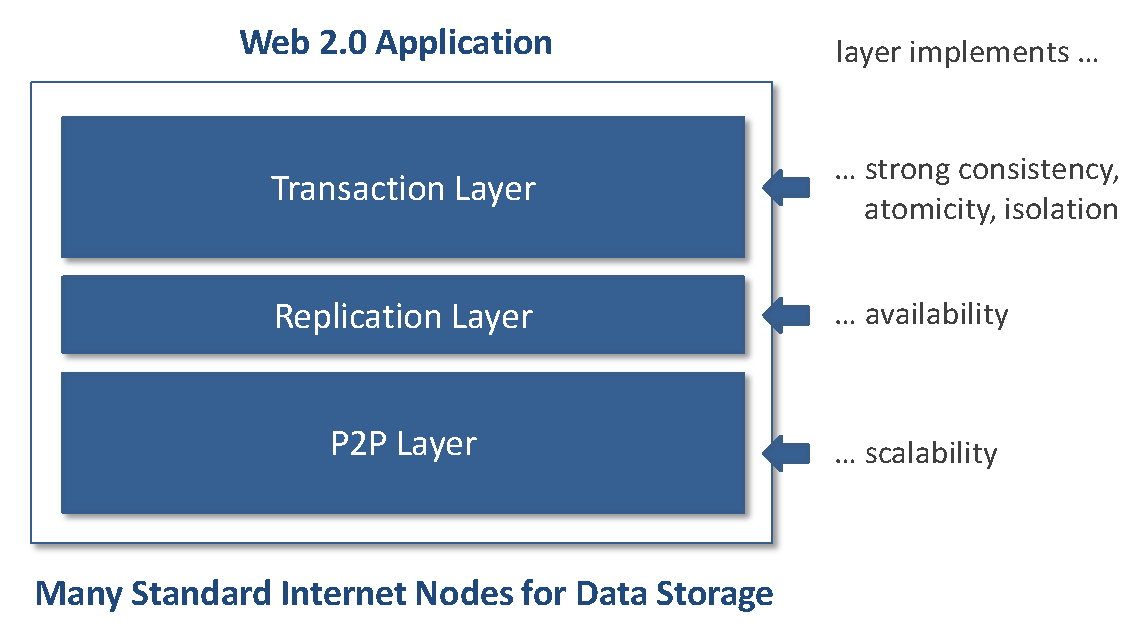
\includegraphics[width=0.7\linewidth]{layers}
\end{center}

\scalaris{} takes care of:

\begin{itemize}
\item Fail-over
\item Data distribution
\item Replication
\item Strong consistency
\item Transactions
\end{itemize}

The \scalaris{} project was initiated by Zuse Institute Berlin and onScale
solutions and was partly funded by the EU projects Selfman and
XtreemOS. Additional information (papers, videos) can be found at
\url{http://www.zib.de/CSR/Projects/scalaris} and
\url{http://www.onscale.de/scalarix.html}.

\section{Brewer's CAP Theorem}

In distributed computing there exists the so called CAP theorem. It
basically says that there are three desirable properties for distributed
systems but one can only have any two of them.

\begin{description}
\item {Strict Consistency.} Any read operation has to return the
  result of the latest write operation on the same data item.

\item {Availability.} Items can be read and modified at any time.

\item {Partition Tolerance.} The network on which the service is
  running may split into several partitions which cannot communicate
  with each other. Later on the networks may re-join again.

  For example, a service is hosted on one machine in Seattle and one
  machine in Berlin. This service is partition tolerant if it can
  tolerate that all Internet connections over the Atlantic (and
  Pacific) are interrupted for a few hours and then get repaired.
\end{description}

The goal of \scalaris{} is to provide strict consistency and partition
tolerance. We are willing to sacrifice availability to make sure that
the stored data is always consistent. I.e. when you are running
\scalaris{} with a replication degree of 4 and the network splits into
two partitions, one partition with three replicas and one partition
with one replica, you will be able to continue to use the service only
in the larger partition. All requests in the smaller partition will
time out until the two networks merge again. Note, most other
key-value stores tend to sacrifice consistency.

\section{Scientific Background}

{\bf Basics.} The general structure of \scalaris{} is modelled after
Chord. The Chord paper~\cite{chord-sigcomm} describes the ring
structure, the routing algorithms, and basic ring maintenance.

The main routines of our Chord node are in \code{src/dht\_node.erl} and
the join protocol is implemented in \code{src/dht\_node\_join.erl} (see
also Chap.~\sieheref{chapter.join}). Our implementation of the routing
algorithms is described in more detail in Sect.~\sieheref{chapter.routing}
and the actual implementation is in \code{src/rt\_chord.erl}.

{\bf Transactions.} The most interesting part is probably the
transaction algorithms. The most current description of the algorithms
and background is in \cite{enhanced-paxos}.

The implementation consists of the paxos algorithm in \code{src/paxos} and
the transaction algorithms itself in \code{src/transactions} (see also
Chap.~\sieheref{chapter.transactions}).

{\bf Ring Maintenance.} We changed the ring maintenance algorithm in
\scalaris{}. It is not the standard Chord one, but a variation of
T-Man~\cite{t-man}. It is supposed to fix the ring structure
faster. In some situations, the standard Chord algorithm is not able
to fix the ring structure while T-Man can still fix it. For node sampling,
our implementation relies on Cyclon~\cite{cyclon}.

The T-Man implementation can be found in \code{src/rm\_tman.erl} and
the Cyclon implementation in \code{src/cyclon}.

{\bf Vivaldi Coordinates.} For some experiments, we implemented so
called Vivaldi coordinates~\cite{vivaldi}. They can be used to
estimate the network latency between arbitrary nodes.

The implementation can be found in \code{src/vivaldi.erl}.

{\bf Gossipping.} For some algorithms, we use estimates of global
information. These estimates are aggregated with the help of
gossipping techniques~\cite{gossip}.

The implementation can be found in \code{src/gossip.erl}.
